% begin module cycloid-area-ex3
\begin{frame}
\begin{example} %[Example 3, p. 668]
\begin{columns}[c]
\column{.5\textwidth}
\psset{xunit=0.6cm, yunit=0.6cm, algebraic=true}
\begin{pspicture}(-1.290703, -0.7)(7.5, 2.8)%
\tiny
\psframe*[linecolor=white](-1.290703, -0.7)(7.5, 2.8)
\pscustom*[linecolor=\fcColorAreaUnderGraph]{%
\parametricplot{0}{6.283185307}{t-sin(t)|1-cos(t)}%
\psline(6.283185307, 0)(0,0)%
}%
\parametricplot[linecolor=\fcColorGraph]{-2}{8.283185307}{t-sin(t)|1-cos(t)}%
\fcAxesStandardNoFrame{-1.090703}{-0.5}{7.373888}{2.5}%
\fcYTickWithLabel{2}{$2r$}
\fcXTickWithLabel{6.283185307}{$2\pi r$}
\end{pspicture}
%\ 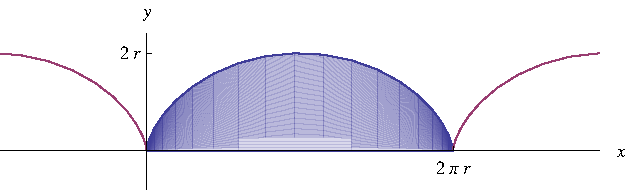
\includegraphics[height=1.7cm]{parametric-curves/pictures/11-02-ex3.pdf}%
\column{.5\textwidth}
Find the area under one arch of the cycloid
\[
\alert<handout:0| 6-7>{x = r(\theta - \sin \theta )},\qquad \alert<handout:0| 4-5>{y = r(1-\cos \theta )}
\]
\end{columns}
\uncover<2->{%
One arch is given by $\alert<handout:0| 8-11>{0\leq \theta \leq 2\pi}$.
}%
\begin{eqnarray*}
\uncover<3->{%
A & = & \int_{\alert<handout:0| 8-9>{0}}^{\alert<handout:0| 10-11>{2\pi r}} \alert<handout:0| 4-5>{y}\alert<handout:0| 6-7>{\diff x}%
} \uncover<4->{ = } \uncover<4->{%
\int_{\alert<handout:0| 8-9>{\uncover<9->{0}}}^{\alert<handout:0| 10-11>{\uncover<11->{2\pi}}} \alert<handout:0| 4-5>{\uncover<5->{r(1-\cos \theta )}}\alert<handout:0| 6-7>{\uncover<7->{r(1-\cos \theta )\diff \theta}}%
}\\%
& \uncover<12->{ = } &%
\uncover<12->{%
r^2 \int_0^{2\pi} (1-\cos \theta )^2\diff \theta%
}  \uncover<13->{ = } \uncover<13->{%
r^2 \int_0^{2\pi} (1-2\cos \theta + \alert<handout:0| 14>{\cos^2 \theta}) \diff \theta%
}\\%
& \uncover<14->{ = } &%
\uncover<14->{%
r^2 \int_0^{2\pi} \left( 1-2\cos \theta + \alert<handout:0| 14>{\frac{1}{2}(1+\cos 2 \theta)}\right) \diff \theta%
}\\%
&  \uncover<15->{ = } &%
\uncover<15->{%
r^2 \left[ \frac{3}{2}\theta -2\sin \theta + \frac{1}{4}\sin 2\theta \right]_0^{2\pi}%
}  \uncover<16->{ = } \uncover<16->{%
r^2 \left( \frac{3}{2} \cdot 2\pi \right) = 3\pi r^2%
}\\%
\end{eqnarray*}
\end{example}
\end{frame}
% end module cycloid-area-ex3
